\subsection{Edge Split}
An edge in parametric space represents a (possible) curve on the
surface. Any edge, with length $L_E$, can have at most the same length
as the portion of the surface which it represents, $L_S$. Therefore, the
representation deficit for an edge, $RD_E$, is defined as $RD_E =
\frac{L_S - L_E}{L_E}$. Note that the lengths are calculated in
${\mathbb R}^3$. The difference in length, $\left(L_S - L_E\right)$, is
normalized by $L_E$ so that the result is scale independent. Also, this
is representation {\it deficit} since $L_S \ge L_E$ is always true.

In order to apply the above definition of representation deficit to mesh
generation, a replacement for $L_S$ must be determined since the length
along the surface represented by $L_S$ is not always able to be
determined -- or, most often, the arc-length calculation is impractical.
Generally, in order to reduce the representation deficit for an edge, the
edge is split by inserting an interior point. Any point that is inserted
into the interior of the edge would decrease the representation deficit
--- or, at worst, it will remain the same. However, the determination of
where to split the edge should be done in such a way that the
representation deficit is minimized. This strategy of refinement,
i.e., refining each edge in such a way that the representation deficit is
locally minimized, would take advantage of the optimal substructure of
the discrete topology. A method for generating a locally optimal edge
split is detailed in \cite{mclaurin12,mclaurin13}.

\begin{figure}[h!]
  \center{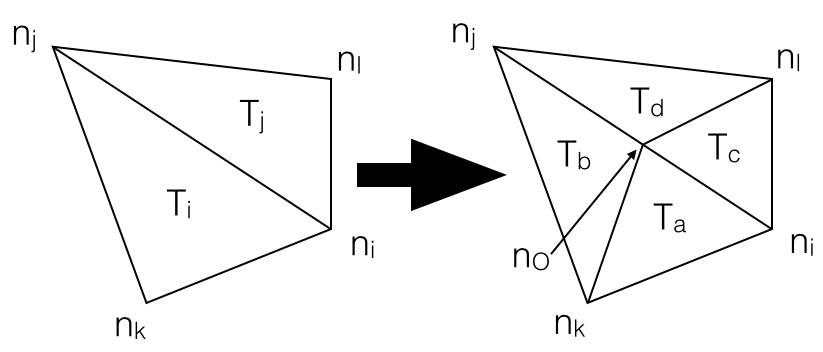
\includegraphics[height=1.4in]
    {Figures/EdgeSplit.jpg}}
  \caption{Edge Split}
\end{figure}

In addition, the fact that an edge split will change the surface area of
the discretization should be considered. Since the overall 
motivation of this work is to reduce the {\it area} representation deficit 
of a discretization, the representation deficit will not be defined for an
edge but for an edge-split. Therefore, for a given edge, only the
edge-split that minimizes {\it area} representation deficit is
considered. The process of determining where to split a triangle is
defined here by locally optimizing an objective function defined for an
edge-split.  Let $E\left(n_i,n_j\right)$ be an edge in $D$ that is
topologically adjacent to two triangles, $T_i\left(n_i,n_j,n_k\right)$
and $T_j\left(n_i,n_l,n_j\right)$. Additionally, let a node on the
interior of the edge be defined as $n_O$. The five nodes,
$\left\{n_i,n_j,n_k,n_l,n_O\right\}$ define four triangles, i.e.,
$T_a\left(n_i,n_O,n_k\right)$, $T_b\left(n_O,n_j, n_k\right)$,
$T_c\left(n_i,n_l,n_O\right)$, $T_d\left(n_O,n_l,n_j\right)$.  The
optimization problem for finding the optimal position for $n_O$ on $E$
is defined as:

\begin{eqnarray*}
\begin{array}{rcl}
\underset{n_O}{\text{minimize}} \ O(E) & = & - \frac{ A\left(T_a\right) + A\left(T_b\right) + A\left(T_c\right) + A\left(T_d\right) }{ A\left(T_i\right) + A\left(T_j\right) } \\
\text{subject to} \ N_{T_a} & > & 0 \\
N_{T_b} & > & 0 \\ 
N_{T_c} & > & 0 \\
N_{T_d} & > & 0. \\
\end{array}
\end{eqnarray*}
